\section{Il caso particolare della briscola in 5}

La briscola in 5 presenta una peculiarità rispetto alla maggir parte degli altri giochi di carte e da tavolo in generale: la suddivisione dei cinque giocatori in due squadre, necessariamente assimetriche, non avviene prima dell'inizio della partita, bensì all'interno della stessa.
Inoltre, i giocatori posseggono una diversa quantità d'informazione riguardante la formazione delle squadre, che per alcuni può rimanere incerta per gran parte della partita.
Per questo è auspicabile considerare le due fasi del gioco separatamente: dapprima vi è una fase in cui la formazione delle squadre non è nota a tutti; una volta che il \emph{socio} gioca la carta chiamata, palesandosi, ha inizio la seconda fase, durante la quale i ruoli di tutti i giocatori diventano chiari.
La seconda fase del gioco quindi non si discosta troppo da altri giochi già molto trattati nell'ambito dell'AI, come il \emph{Bridge}.
Uno studio di \cite{villa} ad esempio, applica a questa fase della briscola in 5 il metodo della ricerca nello spazio degli stati con approssimazione Montecarlo, soluzione già indicata come comune nella risoluzione di giochi di carte.
Non siamo invece riusciti a trovare studi che trattino la prima fase della briscola in 5, quella durante la quale non è chiaro a tutti chi siano gli avversari e chi i compagni.
Infatti, quello della briscola in 5 nella sua prima fase non può essere considerato un ambiente nè \emph{competitivo} nè \emph{cooperativo}.
Questo rende impossibile l'applicazione diretta dei metodi indicati nelle precedenti sezioni così come sono e chiama un approccio di tipo differente.

\subsection{Inapplicabilità di algoritmi di ricerca e teoria dei giochi}
Volendo tentare di applicare l'algoritmo \textsc{Minimax} alla risoluzione di una partita di briscola in 5 ci si scontra immediatamente con una difficoltà insormontabile per l'algoritmo nella sua versione classica: essendo impossibile definire con certezza una funzione di utilità, è inapplicabile la definizione ricorsiva \ref{minimax-value} del \emph{mini-max value}.
Questo accade perchè, pur assumendo di aver costruito l'intero albero rappresentante lo spazio degli stati fino alle foglie che contengono gli stadi finali della partita, è impossibile assegnare un segno, positivo o negativo, al modulo delle funzioni di utilità: esso sarebbe positivo se il giocatore che si aggiudica la presa fosse un compagno, viceversa, sarebbe negativo.
Ma essendo sconosciuto il ruolo del giocatore che ``prende'', rimane incerto il valore della funzione di utilità.\\
Per poter applicare l'approccio \textsc{Minimax} anche in questo scenario, si renderebbe necessario aumentare il numero di mondi possibili, moltiplicandolo per 3 (il numero massimo dei giocatori dei quali non si conosce il ruolo) per considerare tutte le situazioni possibili.
Ma in questo caso, essendo le funzioni di utilità dei differenti mondi diametralmente opposte, sarebbe anche auspicabile possedere delle valide euristiche che permettano di assegnare con buon grado di confidenza una probabilità ad ogni possibile ``mondo terminale'' (ovvero alla possibilità che ognuno dei 3 giocatori di cui non si conosce il ruolo sia il socio).

\subsubsection*{Esempio}
Si può immaginare una situazione in cui un giocatore, $P$, nel ruolo di \emph{villano}, durante la fase in cui il \emph{socio} non si sia ancora rivelato, si trovi ultimo di mano in una partita contro i giocatori $A$, $B$, $C$ e $G$. $G$ sia il \emph{chiamante}.\\
In tavolo non vi siano briscole; il seme regnante sia $\heartsuit$.\\
La presa spetti al giocatore, $A$ del quale ancora non si conosce il ruolo.\\
$A$ prenda con un Asso di $\heartsuit$.\\
In tavolo vi siano anche: K $\heartsuit$, J $\diamondsuit$, 2 $\spadesuit$.\\
Il seme di briscola sia $\clubsuit$.\\
In mano si abbiano 2 $\clubsuit$ e 2 $\heartsuit$ : una briscola ed un liscio.\\
Immaginiamo, per facilitare i calcoli, che quasi tutti i punti siano già stati giocati e che rimanga una sola mano da giocarsi con un punteggio inferiore a quello in tavola.\\
In una situazione del genere un giocatore umano incerto sui ruoli degli altri giocatori giocherebbe certamente la briscola (quindi il 2 $\clubsuit$), aggiudicandosi la mano senza per questo dover rinunciare a dei punti.\\
Ma la situazione è utile per mostrare l'inapplicabilità della definizione del \emph{minimax value}: se si decidesse di giocare il 2 $\heartsuit$, infatti, i punti raccolti dal giocatore $A$ che ha giocato A $\heartsuit$, sarebbero a proprio vantaggio o svantaggio?\\
Giocando il 2 $\clubsuit$ si è certi che, qualsiasi sia lo svolgersi della mano successiva, il punteggio della propria squadra aumenterà di 16 punti.\\
Giocando il 2 $\heartsuit$, invece, i 16 punti della mano potrebbero essere a favore della propria squadra come di quella avversaria, in base all'affiliazione del giocatore che si aggiudica la presa.\\
Allo stesso tempo, se il giocatore \emph{P} fosse sicuro di essere in squadra con \emph{A}, dovrebbe certamente ``andare liscio'' giocando il 2 $\heartsuit$, mantenendo in mano in questo modo una briscola che potrebbe rivelarsi molto utile nella mano successiva (anche se in questo caso abbiamo ipotizzato, per semplificare, che tutti i punti siano già stati giocati).


\begin{figure}[!htbp]
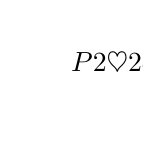
\begin{tikzpicture}
\tikzset{every tree node/.style={align=center,anchor=north}}
\tikzset{level 1/.style={level distance=70pt}}
\tikzset{level 2/.style={level distance=35pt}}
\tikzset{level 3/.style={level distance=35pt}}
\tikzset{level 4/.style={level distance=45pt}}
\tikzset{level 5/.style={level distance=20pt}}


\Tree[.{$P$ ha in mano \\ $2  \heartsuit$ e $ 2  \clubsuit$}
         [.{$P$ gioca $2 \heartsuit$} [ .{\ldots} [.{termine partita} [ .{Il socio è A} [\node [draw, circle] { - 16}; ] ] [ .{Il socio è B}  [ \node [draw, circle] {+ 16}; ]] [ .{Il socio è C}  [ \node [draw, circle] {+ 16}; ]] ]]]
         [.{$P$ gioca $2 \clubsuit$} [ .{\ldots} [.{termine partita} [ .{Il socio è A}  [ \node [draw, circle] {+ 16}; ]] [ .{Il socio è B}  [ \node [draw, circle] {+ 16}; ]] [ .{Il socio è C}  [ \node [draw, circle] {+ 16}; ]] ]]]
]
\end{tikzpicture}

\caption{Valori indefiniti per la utility function}
\label{alberoutility}
\end{figure}

\subsection*{}

Come è stato detto, l'applicazione del modello della teoria dei giochi alla Briscola in 5 richiede comunque lo sviluppo di un albero di decisione; oltre ai già trattati (e superabili) problemi di estensione di tale albero, il problema descritto in \ref{alberoutility} si ripresenta nel momento in cui si voglia applicare il modello della teoria dei giochi a un ambiente come quello della Briscola in 5 che non è definitamente nè competitivo nè cooperativo.\\
Esattamente come i valori della \emph{utility function} usati dall'algoritmo \textsc{Minimax}, anche i \emph{payoff} necessari alla realizzazione della forma estesa del gioco della Briscola in 5 non sarebbero definibili se non conoscendo in anticipo la formazione delle squadre.


\subsection{Soluzione adottata}

Per le difficoltà di cui sopra, si è deciso di scartare per ora un approccio puramente algoritmico per la soluzione.
Si è invece optato per gestire la fase di gioco tentando di simulare i comportamenti umani di giocatori esperti.
Questo viene fatto sia mettendo a disposizione un insieme di strategie basilari all'interno di un framework appositamente pensato per facilitare la scrittura delle stesse, sia proponendo un sistema che permetta all'utente esperto di suggerire nuove strategie per l'ampliamento, l'integrazione e la modifica di quelle pre-esistenti.\\
L'utilizzo di questo tipo di approccio per la prima fase del gioco non esclude la possibilità di integrarlo con metodi di soluzione più classici come quelli accennati nelle precedenti sezioni: inadatti alla prima fase della partita, questi potrebbero infatti benissimo essere usati per la soluzione della seconda, una volta che le squadre siano a tutti note.
